%----------------------------------------------------------------------------------------
% The original JLA LaTeX template has been modified by JooYoung Seo (jooyoung@psu.edu) to work with R Markdown.
%----------------------------------------------------------------------------------------

%%%%%%%%%%%%%%%%%%%%%%%%%%%%%%%%%%%%%%%%%
% Stylish Article
% LaTeX Template
% Version 2.1 (1/10/15)
%
% This template has been downloaded from:
% http://www.LaTeXTemplates.com
%
% Original author:
% Mathias Legrand (legrand.mathias@gmail.com) 
% With extensive modifications by:
% Vel(vel@latextemplates.com)
%
% License:
% CC BY-NC-SA 3.0 (http://creativecommons.org/licenses/by-nc-sa/3.0/)
%
%%%%%%%%%%%%%%%%%%%%%%%%%%%%%%%%%%%%%%%%%

%----------------------------------------------------------------------------------------
%	PACKAGES AND OTHER DOCUMENT CONFIGURATIONS
%----------------------------------------------------------------------------------------

\documentclass[fleqn,10pt]{JLA_article} % Document font size and equations flushed left

\usepackage[english]{babel} % Specify a different language here - english by default

%\usepackage{lipsum} % Required to insert dummy text. To be removed otherwise


%----------------------------------------------------------------------------------------
%	HYPERLINKS
%----------------------------------------------------------------------------------------

\usepackage{hyperref} % Required for hyperlinks
\hypersetup{hidelinks,colorlinks,breaklinks=true,urlcolor=color2,citecolor=color1,linkcolor=color1,bookmarksopen=false,pdftitle={Title},pdfauthor={Author}}

%----------------------------------------------------------------------------------------
%	ARTICLE INFORMATION
%----------------------------------------------------------------------------------------

\PaperTitle{JLA Article Template} % Article title

\Authors{JooYoung Seo\textsuperscript{1}, Arang Seo\textsuperscript{2}, First M. Last\textsuperscript{3}} % Authors
\affiliation{Corresponding author \textsuperscript{1}\textit{Email: \href{mailto:jooyoung@psu.edu}{\nolinkurl{jooyoung@psu.edu}} Learning, Design, and Technology, 301 Keller Building, University Park, PA 16802, USA, \url{https://orcid.org/0000-0002-4064-6012}}\\\textsuperscript{2}\textit{Email: \href{mailto:sjysky@gmail.com}{\nolinkurl{sjysky@gmail.com}} Department of Education, Guidedog University, Yongin-Si, Republic of Korea, if available}\\\textsuperscript{3}\textit{Email: \href{mailto:somebody@example.com}{\nolinkurl{somebody@example.com}} Department of Computer Science, Example University,Street, Building, Postal Code, City, Country, if available}} % Author affiliation

\Keywords{Include a set of keywords related to your submission. Separate them by commas.} 

\Submitted{25/04/20}
\Accepted{dd/mm/yy}
\Published{dd/mm/yy}

\Volume{1}
\Number{1}
\Pages{1---10}
\Doi{xxx-xxx-xxx}
%----------------------------------------------------------------------------------------
%	NOTES FOR PRACTICE OR RESEARCH
%----------------------------------------------------------------------------------------

\Notesname{Notes for Practice} %If this is a Research Paper
%\Notesname{Notes for Research} %If this is a Practitioner Paper

\note{This is an example of a note to practice or research.}
\note{This is a second example of a note to practice or research.}
\note{This is a third example of a note to practice or research.}

%----------------------------------------------------------------------------------------
%	ABSTRACT
%----------------------------------------------------------------------------------------

\Abstract{Abstracts shall not exceed 200 words. Do not use a heading for the abstract or headings within the abstract.}

%----------------------------------------------------------------------------------------

% Pandoc syntax highlighting



\begin{document}

\flushbottom % Makes all text pages the same height

\maketitle % Print the title and abstract box

%\tableofcontents % Print the contents section

\thispagestyle{fancy} % Add header to first page

\hypertarget{introduction}{%
\section{Introduction}\label{introduction}}

This is example text. Note that JLA uses up to 3 levels of headings (e.g.~1., 1.1, 1.1.1). Please do not add additional levels beyond the three that have been provided.

This is an example of including math \(\cos\pi=-1\) and \(\alpha\) directly within the text\footnote{And an example of a footnote including math $\cos\pi=-1$ and $\alpha$ in the text.}.

Important formulas should be presented on a seperate line as shown in the next section (See Formula 1).

All figures and tables should be explicitly referenced in the appropriate part of the text (See Table 1 and Figure 2).

This template use the \href{http://ctan.uniminuto.edu/biblio/bibtex/contrib/apacite/apacite.pdf}{apacite package}.

This is an example on how to cite (Figueredo and Wolf 2009). Here is a citation when you want to address the authors directly, for example the work of Archambault et al. (2009).

\hypertarget{table-test}{%
\subsection{Table Test}\label{table-test}}

Table~\ref{tab:test} shows an example below:

\begin{table}

\caption{\label{tab:test}Test table.}
\centering
\begin{tabular}[t]{r|r|r|r|l}
\hline
Sepal.Length & Sepal.Width & Petal.Length & Petal.Width & Species\\
\hline
5.1 & 3.5 & 1.4 & 0.2 & setosa\\
\hline
4.9 & 3.0 & 1.4 & 0.2 & setosa\\
\hline
4.7 & 3.2 & 1.3 & 0.2 & setosa\\
\hline
4.6 & 3.1 & 1.5 & 0.2 & setosa\\
\hline
5.0 & 3.6 & 1.4 & 0.2 & setosa\\
\hline
5.4 & 3.9 & 1.7 & 0.4 & setosa\\
\hline
\end{tabular}
\end{table}

\hypertarget{figure-test}{%
\subsection{Figure Test}\label{figure-test}}

See Figure~\ref{fig:hist} for example.

\begin{figure}
\centering
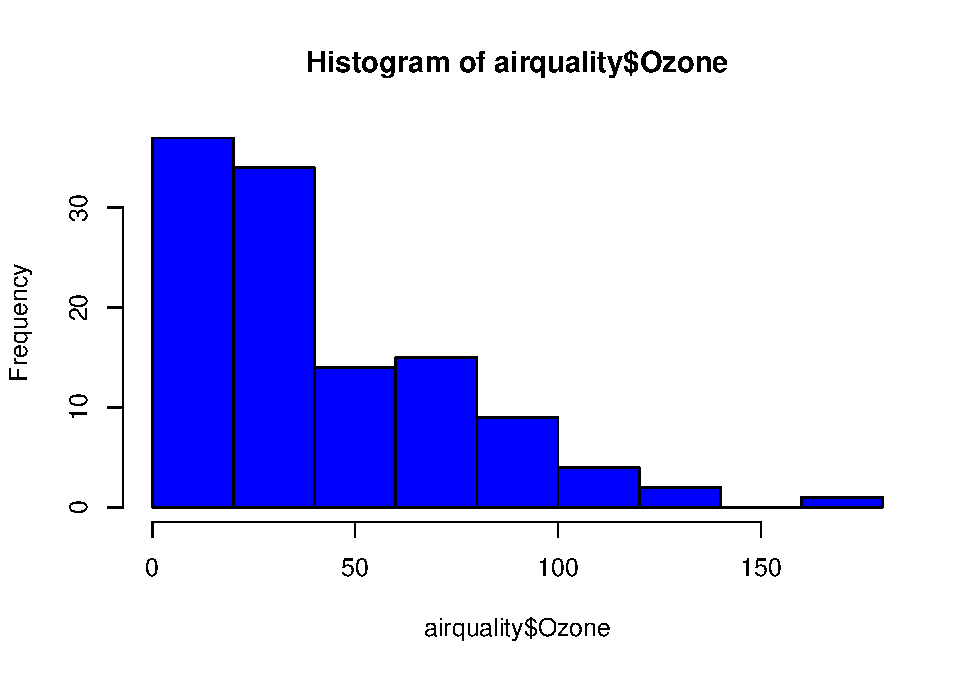
\includegraphics{fig/hist-1.pdf}
\caption{\label{fig:hist}Histogram of ozone.}
\end{figure}

\hypertarget{literature-review}{%
\section{Literature Review}\label{literature-review}}

Lorem ipsum dolor sit amet, consectetur adipiscing elit. Pellentesque rhoncus ut tellus eu tristique. Duis pharetra velit vitae viverra elementum. Nulla metus dui, pulvinar id enim at, pellentesque semper ipsum. Phasellus cursus dignissim ipsum, sed congue orci pretium quis. Maecenas rhoncus leo a cursus euismod. Fusce a erat eu ipsum tristique tempus at sed tortor. Aliquam erat volutpat. Donec at pretium lorem. Donec pretium nunc id nunc bibendum convallis. Phasellus quis enim id massa feugiat egestas hendrerit sollicitudin nibh. Sed blandit eros id tellus porta, eget ullamcorper urna posuere. Pellentesque laoreet lacus nibh, a mattis libero viverra sit amet. Sed vitae diam interdum, pharetra neque sit amet, dictum lectus.

Donec massa justo, ultricies quis facilisis sed, tristique nec metus. Vestibulum id condimentum diam. Integer semper augue id porttitor ultrices. Cras vulputate felis eu diam porttitor, ac pulvinar nisi imperdiet. Donec eros felis, imperdiet vel malesuada at, varius et quam. Phasellus facilisis non risus eu placerat. Sed ac mollis lorem.

\hypertarget{methods}{%
\section{Methods}\label{methods}}

\begin{figure}[ht]\centering % Using \begin{figure*} makes the figure take up the entire width of the page
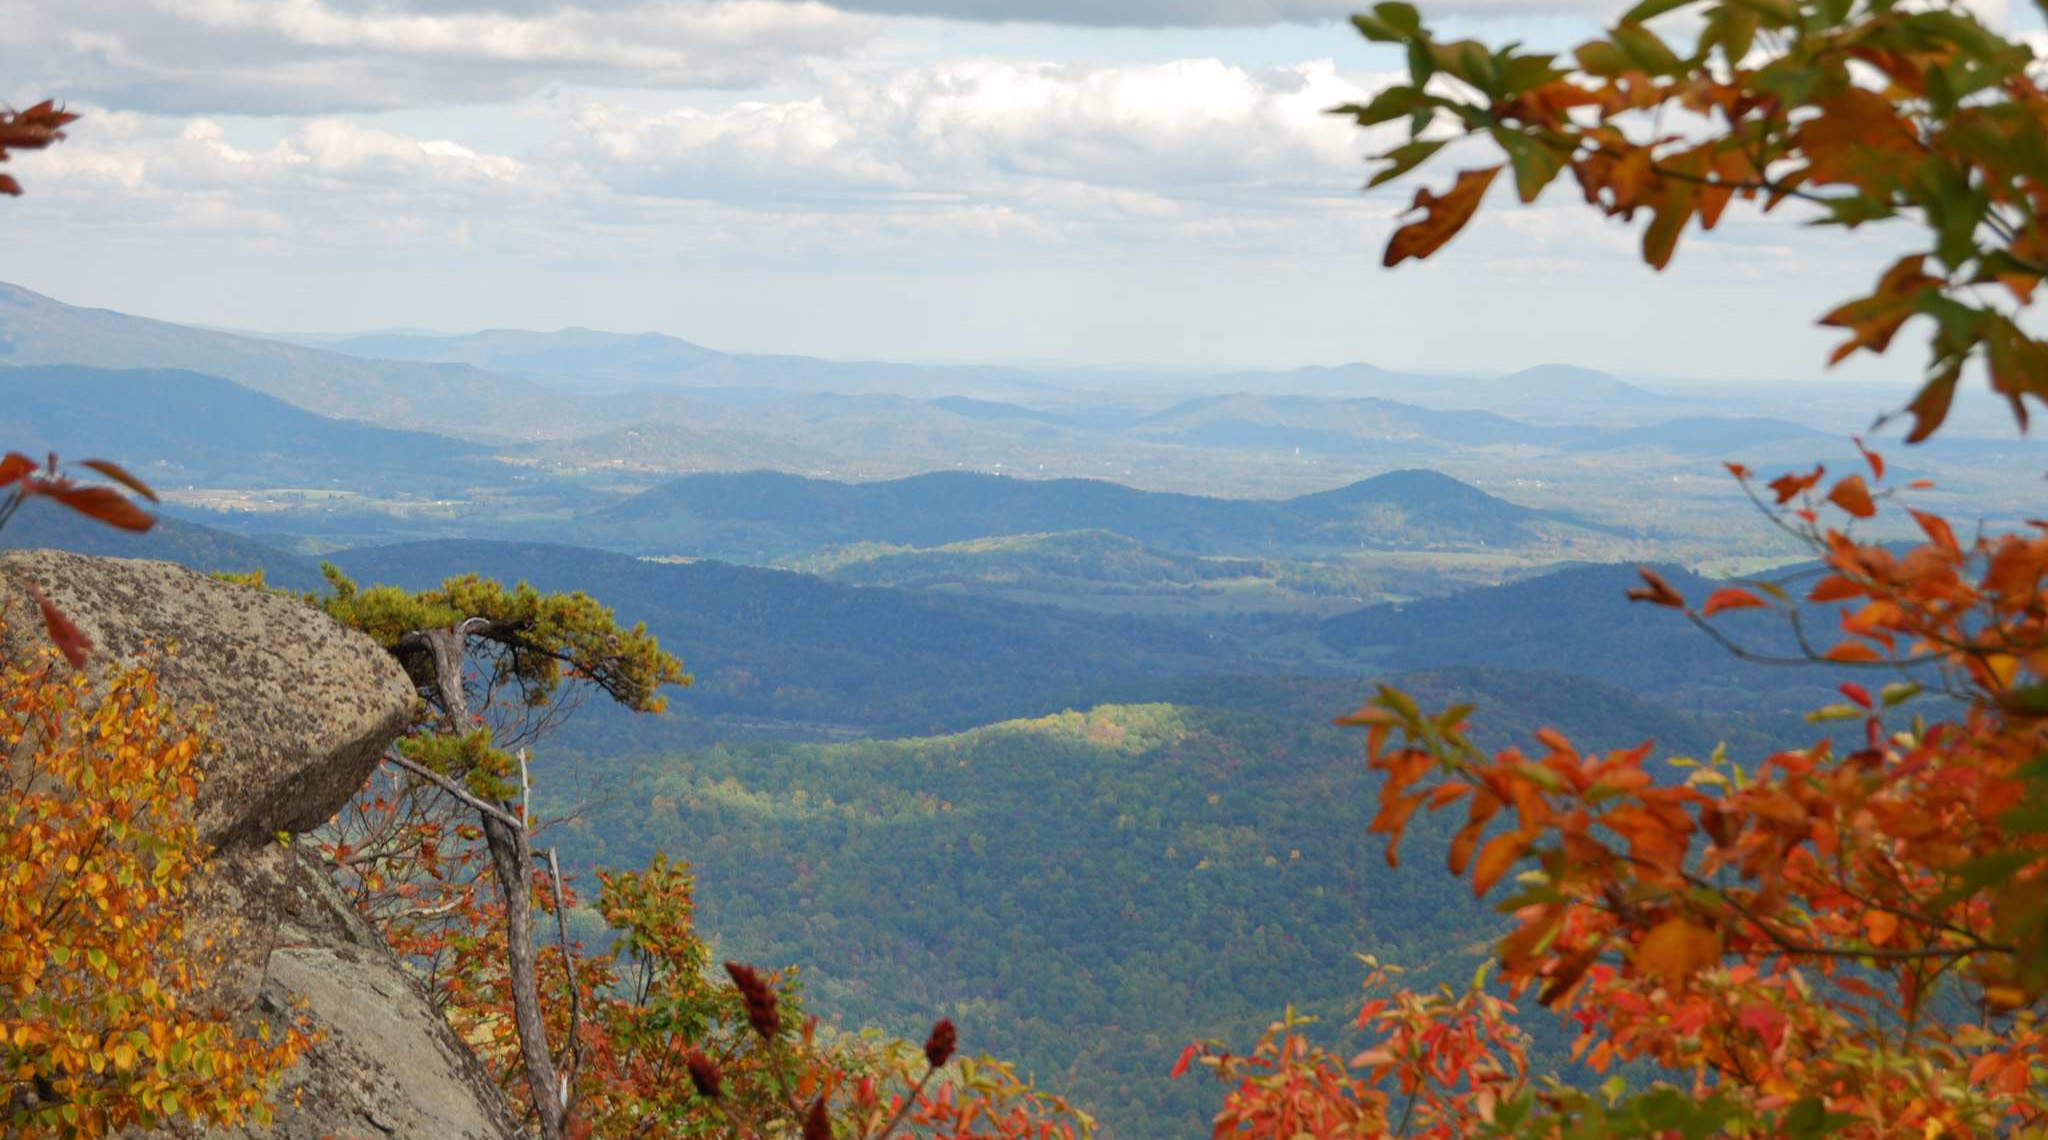
\includegraphics[width=\linewidth/2]{fig/view}
\caption{Picture}
\label{fig:view}
\end{figure}

\begin{equation}
\cos^3 \theta =\frac{1}{4}\cos\theta+\frac{3}{4}\cos 3\theta
\label{eq:refname2}
\end{equation}

\begin{enumerate}[noitemsep] % [noitemsep] removes whitespace between the items for a compact look
\item First item in a list
\item Second item in a list
\item Third item in a list
\end{enumerate}

\hypertarget{subsection}{%
\subsection{Subsection}\label{subsection}}

Nullam semper imperdiet orci, at lacinia est aliquet et. Sed justo nibh, aliquet et velit at, pharetra consequat velit. Nullam nec ligula sagittis, adipiscing nisl sed, varius massa. Mauris quam ante, aliquet a nunc et, faucibus imperdiet libero. Suspendisse odio tortor, bibendum vel semper sit amet, euismod ac ante. Nunc nec dignissim turpis, ac blandit massa. Donec auctor massa ac vestibulum aliquam. Fusce auctor dictum lobortis. Vivamus tortor augue, convallis quis augue sit amet, laoreet tristique quam. Donec id volutpat orci. Suspendisse at mi vel elit accumsan porta ac ut diam. Nulla ut dapibus quam.

Sed est odio, ornare in rutrum et, dapibus in urna. Suspendisse varius massa in ipsum placerat, quis tristique magna consequat. Suspendisse non convallis augue. Quisque fermentum justo et lorem volutpat euismod. Vestibulum ante ipsum primis in faucibus orci luctus et ultrices posuere cubilia Curae; Morbi sagittis interdum justo, eu consequat nisi convallis in. Sed tincidunt risus id lacinia ultrices. Phasellus ac ligula sed mi mattis lacinia ac non felis. Etiam at dui tellus.

\hypertarget{subsection-1}{%
\subsection{Subsection}\label{subsection-1}}

Nullam semper imperdiet orci, at lacinia est aliquet et. Sed justo nibh, aliquet et velit at, pharetra consequat velit. Nullam nec ligula sagittis, adipiscing nisl sed, varius massa. Mauris quam ante, aliquet a nunc et, faucibus imperdiet libero. Suspendisse odio tortor, bibendum vel semper sit amet, euismod ac ante. Nunc nec dignissim turpis, ac blandit massa. Donec auctor massa ac vestibulum aliquam. Fusce auctor dictum lobortis. Vivamus tortor augue, convallis quis augue sit amet, laoreet tristique quam. Donec id volutpat orci. Suspendisse at mi vel elit accumsan porta ac ut diam. Nulla ut dapibus quam.

Sed est odio, ornare in rutrum et, dapibus in urna. Suspendisse varius massa in ipsum placerat, quis tristique magna consequat. Suspendisse non convallis augue. Quisque fermentum justo et lorem volutpat euismod. Vestibulum ante ipsum primis in faucibus orci luctus et ultrices posuere cubilia Curae; Morbi sagittis interdum justo, eu consequat nisi convallis in. Sed tincidunt risus id lacinia ultrices. Phasellus ac ligula sed mi mattis lacinia ac non felis. Etiam at dui tellus.

\begin{figure}[ht]\centering
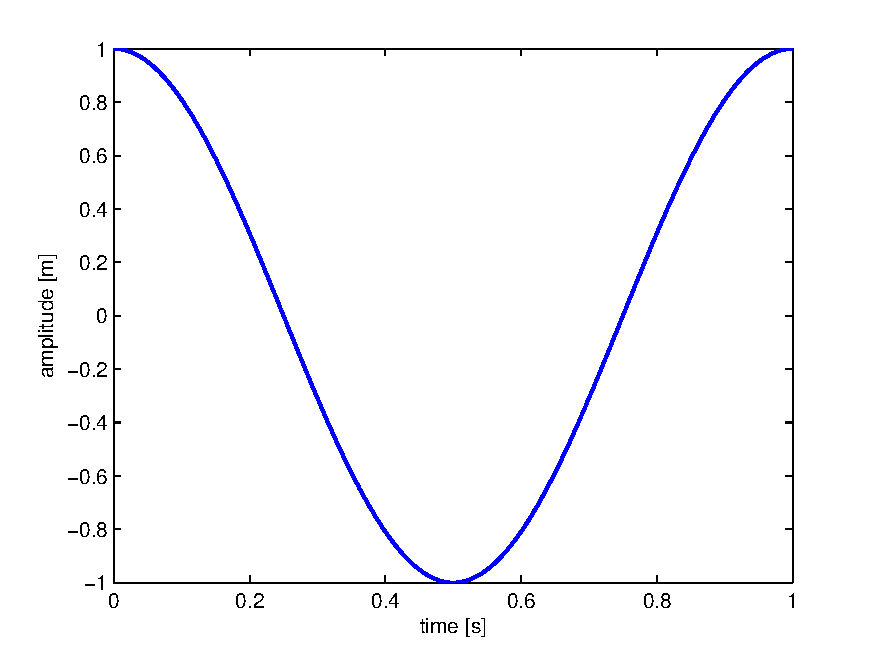
\includegraphics[width=\linewidth/2]{fig/results}
\caption{In-text Picture}
\label{fig:results}
\end{figure}

Reference to Figure \ref{fig:results}.

\hypertarget{results-and-discussion}{%
\section{Results and Discussion}\label{results-and-discussion}}

Nullam semper imperdiet orci, at lacinia est aliquet et. Sed justo nibh, aliquet et velit at, pharetra consequat velit. Nullam nec ligula sagittis, adipiscing nisl sed, varius massa. Mauris quam ante, aliquet a nunc et, faucibus imperdiet libero. Suspendisse odio tortor, bibendum vel semper sit amet, euismod ac ante. Nunc nec dignissim turpis, ac blandit massa. Donec auctor massa ac vestibulum aliquam. Fusce auctor dictum lobortis. Vivamus tortor augue, convallis quis augue sit amet, laoreet tristique quam. Donec id volutpat orci. Suspendisse at mi vel elit accumsan porta ac ut diam. Nulla ut dapibus quam.

Sed est odio, ornare in rutrum et, dapibus in urna. Suspendisse varius massa in ipsum placerat, quis tristique magna consequat. Suspendisse non convallis augue. Quisque fermentum justo et lorem volutpat euismod. Vestibulum ante ipsum primis in faucibus orci luctus et ultrices posuere cubilia Curae; Morbi sagittis interdum justo, eu consequat nisi convallis in. Sed tincidunt risus id lacinia ultrices. Phasellus ac ligula sed mi mattis lacinia ac non felis. Etiam at dui tellus.

\hypertarget{subsection-2}{%
\subsection{Subsection}\label{subsection-2}}

\begin{table}[hbt]
\caption{Table of Grades}
\centering
\begin{tabular}{llr}
\toprule
\multicolumn{2}{c}{Name} \\
\cmidrule(r){1-2}
First name & Last Name & Grade \\
\midrule
John & Doe & $7.5$ \\
Richard & Miles & $2$ \\
\bottomrule
\end{tabular}
\label{tab:label}
\end{table}

\hypertarget{subsubsection}{%
\subsubsection{Subsubsection}\label{subsubsection}}

Nullam semper imperdiet orci, at lacinia est aliquet et. Sed justo nibh, aliquet et velit at, pharetra consequat velit. Nullam nec ligula sagittis, adipiscing nisl sed, varius massa. Mauris quam ante, aliquet a nunc et, faucibus imperdiet libero. Suspendisse odio tortor, bibendum vel semper sit amet, euismod ac ante. Nunc nec dignissim turpis, ac blandit massa. Donec auctor massa ac vestibulum aliquam. Fusce auctor dictum lobortis. Vivamus tortor augue, convallis quis augue sit amet, laoreet tristique quam. Donec id volutpat orci. Suspendisse at mi vel elit accumsan porta ac ut diam. Nulla ut dapibus quam.

Sed est odio, ornare in rutrum et, dapibus in urna. Suspendisse varius massa in ipsum placerat, quis tristique magna consequat. Suspendisse non convallis augue. Quisque fermentum justo et lorem volutpat euismod. Vestibulum ante ipsum primis in faucibus orci luctus et ultrices posuere cubilia Curae; Morbi sagittis interdum justo, eu consequat nisi convallis in. Sed tincidunt risus id lacinia ultrices. Phasellus ac ligula sed mi mattis lacinia ac non felis. Etiam at dui tellus.

\begin{description}
\item[Word] Definition
\item[Concept] Explanation
\item[Idea] Text
\end{description}

\hypertarget{subsubsection-1}{%
\subsubsection{Subsubsection}\label{subsubsection-1}}

\begin{itemize}[noitemsep] % [noitemsep] removes whitespace between the items for a compact look
\item First item in a list
\item Second item in a list
\item Third item in a list
\end{itemize}

\hypertarget{subsubsection-2}{%
\subsubsection{Subsubsection}\label{subsubsection-2}}

Nullam semper imperdiet orci, at lacinia est aliquet et. Sed justo nibh, aliquet et velit at, pharetra consequat velit. Nullam nec ligula sagittis, adipiscing nisl sed, varius massa. Mauris quam ante, aliquet a nunc et, faucibus imperdiet libero. Suspendisse odio tortor, bibendum vel semper sit amet, euismod ac ante. Nunc nec dignissim turpis, ac blandit massa. Donec auctor massa ac vestibulum aliquam. Fusce auctor dictum lobortis. Vivamus tortor augue, convallis quis augue sit amet, laoreet tristique quam. Donec id volutpat orci. Suspendisse at mi vel elit accumsan porta ac ut diam. Nulla ut dapibus quam.

Sed est odio, ornare in rutrum et, dapibus in urna. Suspendisse varius massa in ipsum placerat, quis tristique magna consequat. Suspendisse non convallis augue. Quisque fermentum justo et lorem volutpat euismod. Vestibulum ante ipsum primis in faucibus orci luctus et ultrices posuere cubilia Curae; Morbi sagittis interdum justo, eu consequat nisi convallis in. Sed tincidunt risus id lacinia ultrices. Phasellus ac ligula sed mi mattis lacinia ac non felis. Etiam at dui tellus.

\hypertarget{conclusion}{%
\section{Conclusion}\label{conclusion}}

Nullam semper imperdiet orci, at lacinia est aliquet et. Sed justo nibh, aliquet et velit at, pharetra consequat velit. Nullam nec ligula sagittis, adipiscing nisl sed, varius massa. Mauris quam ante, aliquet a nunc et, faucibus imperdiet libero. Suspendisse odio tortor, bibendum vel semper sit amet, euismod ac ante. Nunc nec dignissim turpis, ac blandit massa. Donec auctor massa ac vestibulum aliquam. Fusce auctor dictum lobortis. Vivamus tortor augue, convallis quis augue sit amet, laoreet tristique quam. Donec id volutpat orci. Suspendisse at mi vel elit accumsan porta ac ut diam. Nulla ut dapibus quam.

Sed est odio, ornare in rutrum et, dapibus in urna. Suspendisse varius massa in ipsum placerat, quis tristique magna consequat. Suspendisse non convallis augue. Quisque fermentum justo et lorem volutpat euismod. Vestibulum ante ipsum primis in faucibus orci luctus et ultrices posuere cubilia Curae; Morbi sagittis interdum justo, eu consequat nisi convallis in. Sed tincidunt risus id lacinia ultrices. Phasellus ac ligula sed mi mattis lacinia ac non felis. Etiam at dui tellus.

\hypertarget{acknowledgments}{%
\section*{Acknowledgments}\label{acknowledgments}}
\addcontentsline{toc}{section}{Acknowledgments}

Duis nec purus sed neque porttitor tincidunt vitae quis augue. Donec porttitor aliquam ante, nec convallis nisl ornare eu. Morbi ut purus et justo commodo dignissim et nec nisl. Donec imperdiet tellus dolor, vel dignissim risus venenatis eu. Aliquam tempor imperdiet massa, nec fermentum tellus sollicitudin vulputate. Integer posuere porttitor pharetra. Praesent vehicula elementum diam a suscipit. Morbi viverra velit eget placerat pellentesque. Nunc congue augue non nisi ultrices tempor.

\hypertarget{declaration-of-conflicting-interest}{%
\section*{Declaration of Conflicting Interest}\label{declaration-of-conflicting-interest}}
\addcontentsline{toc}{section}{Declaration of Conflicting Interest}

The author(s) declared no potential conflicts of interest with respect to the research, authorship, and/or publication of this article.

\hypertarget{funding}{%
\section*{Funding}\label{funding}}
\addcontentsline{toc}{section}{Funding}

This study was financially supported by Company X.

\hypertarget{references}{%
\section*{References}\label{references}}
\addcontentsline{toc}{section}{References}

\hypertarget{refs}{}
\leavevmode\hypertarget{ref-archambault2009student}{}%
Archambault, Isabelle, Michel Janosz, Jean-Sébastien Fallu, and Linda S Pagani. 2009. ``Student Engagement and Its Relationship with Early High School Dropout.'' \emph{Journal of Adolescence} 32 (3). Elsevier: 651--70.

\leavevmode\hypertarget{ref-Figueredo:2009dg}{}%
Figueredo, A. J., and P. S. A. Wolf. 2009. ``Assortative Pairing and Life History Strategy - a Cross-Cultural Study.'' \emph{Human Nature} 20: 317--30.

\leavevmode\hypertarget{ref-archambault2009student}{}%
Archambault, Isabelle, Michel Janosz, Jean-Sébastien Fallu, and Linda S Pagani. 2009. ``Student Engagement and Its Relationship with Early High School Dropout.'' \emph{Journal of Adolescence} 32 (3). Elsevier: 651--70.

\leavevmode\hypertarget{ref-Figueredo:2009dg}{}%
Figueredo, A. J., and P. S. A. Wolf. 2009. ``Assortative Pairing and Life History Strategy - a Cross-Cultural Study.'' \emph{Human Nature} 20: 317--30.

\bibliography{bib/sample.bib}

\end{document}
